A pesar de la gran cantidad de bases de datos SQL, también hay una tendencia hacia NoSQL. Las bases de datos NoSQL permiten almacenar datos no estructurados y heterogéneos. La \gls{escalabilidad} mejorada ha ayudado a aumentar su popularidad en mayor medida en el mercado actual. El escalado horizontal significa que la organización no tiene que preocuparse por la infraestructura subyacente. Las bases de datos NoSQL son una alternativa emergente a las bases de datos relacionales más utilizadas. Como su nombre lo indica, no reemplaza completamente a SQL, sino que lo complementa de tal manera que puedan coexistir.
\vspace{0.8cm}

\begin{table}[H]
  \renewcommand{\arraystretch}{1.5}
  \centering
  \scriptsize
  \begin{tabular}{ |p{2cm}||p{5cm}|p{5cm}|  }
    \hline
      & SQL
      & NoSQL \\
    \hline
    Tipo
      & Relacional
      & Distribuido \\
    \hline
    Datos
      & Datos estructurados almacenados en tablas 
      & Datos no estructurados almacenados en archivos JSON \\
    \hline
    Esquema 
      & Estático o predefinido
      & Dinámico \\
    \hline
    Escalable 
      & Vertical
      & Horizontal \\
    \hline
    Consultas
      & Adecuado para consultas complejas 
      & Lenguaje de consulta no estructurado \\
    \hline
    Flexible
      & Esquema rígido ligado a la relación 
      & Esquema adecuado para almacenamiento jerárquico \\
    \hline
    Elasticidad
      & Requiere tiempo de inactividad en la mayoría de los casos 
      & Automática, no requiere interrupción \\
    \hline
  \end{tabular}
  \caption{Comparativa SQL y NoSQL}
\end{table}
\vspace{0.8cm}

El concepto de NoSQL se desarrolló hace mucho tiempo, pero fue después de la introducción de la base de datos como servicio (DBaaS) que obtuvo un reconocimiento destacado. Debido a la alta \gls{escalabilidad} proporcionada por NoSQL, fue visto como un importante competidor del modelo de base de datos relacional. A diferencia de las bases de datos relacionales (RDB), las bases de datos NoSQL están diseñadas para escalar fácilmente a medida que crecen. La mayoría de los sistemas NoSQL han eliminado el soporte multiplataforma y algunas características adicionales innecesarias de RDBMS, haciéndolos mucho más livianos y eficientes que sus contrapartes RDBMS.


\subsection{Orientado a documentos}
El concepto principal de una base de datos orientada a documentos es que el documento contiene grandes cantidades de datos que pueden estar disponibles de manera útil. Se puede acceder a estos documentos como un directorio regular en el que puede tener diferentes colecciones y cada colección tiene documentos que contienen la información deseada. Además, cada colección puede tener colecciones internas. Puede tener un árbol completo de documentos, sin embargo, esta práctica no se recomienda y debe evitar tener más de tres niveles de anidamiento. 
\vspace{0.8cm}

Las bases de datos NoSQL no son necesariamente bases de datos relacionales. Los datos no son representados en términos de filas y columnas de tablas. En MongoDB, los datos se visualizan como objetos o documentos. Esto ayuda a un programador a evitar una capa de traducción, por lo que no es necesario convertir o asignar los objetos con los que trata el código en tablas relacionales. Dichas traducciones se denominan capas de Mapeo Relacional de Objetos (ORM).
\begin{figure}[H]
  \centering
  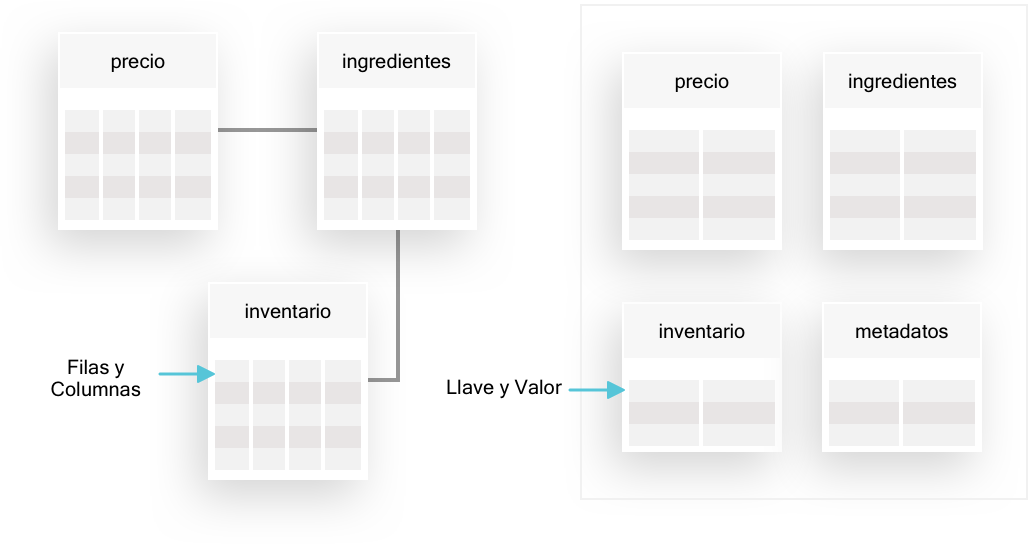
\includegraphics[width=1\textwidth]{sql-nosql}
  \caption{Diagrama que representa las diferencias clave entre la base de datos SQL y las bases de datos NoSQL.}
\end{figure}